\chapter{GÉNÉRALITÉS}
\chaptermark{GÉNÉRALITÉS}
Dans ce chapitre, nous posons les bases en rappelant plusieurs définitions et propriétés importantes vues dans \cite{Di2} et liées à divers concepts de notre étude. Parmi ces éléments,
nous explorons les structures algébriques notamment les anneaux et les modules. Ensuite, nous définissons et classifions les différentes types de filtrations. De plus, nous récapitulons quelques résultats importants associés aux filtrations I-bonnes et présentations un lien entre les filtrations I-bonnes et les autres classes de filtrations. \\\\ Dans l'ensemble de ce mémoire, sauf mention contraire, les anneaux considérés sont supposés \text{commutatifs et unitaires}.
\section{Relation d'équivalences, groupe et sous-groupe}
\subsection{Relation d'équivalences}
\begin{madefinition}
	On appelle relation d’équivalences sur un ensemble non vide E, une relation
	$\Re $ sur E vérifiant les conditions suivantes :
	\begin{enumerate}
		\item[a)] $\forall x \in E, x\Re x$ ;
		\item[b)] $\forall x,y \in E, x\Re y \Longrightarrow y\Re x $;
		\item[c)] $\forall x,y,z \in E,$ [$x\Re y$ et $y\Re z$] $\Longrightarrow (x\Re z)$.
	\end{enumerate}
	La partie $C_x = \{y \in E,\; x\Re y\}  $ de E est appelée la classe d’équivalence modulo $\Re $ de $x \in E$. Les	classes d’équivalence constituent une partition de E. Notons $\mathcal{P}(E)$ l’ensemble des parties de E. La famille $(C_x)_{x \in E}$ constituant $\mathcal{P}(E)$ est appelée l’ensemble quotient de E par $\Re$. On le note $E/\Re $. 
	Dans la suite, la classe de $x \in E$ sera vue essentiellement comme élément de ce nouvel ensemble $E/\Re $ et sera notée $\bar{x}$.
\end{madefinition}
\newpage
\subsection{Relation d'ordre}
\begin{madefinition}
	On appelle relation d’ordre sur un ensemble non vide E, une relation
	$\Re $ sur E vérifiant les conditions suivantes :
	\begin{enumerate}
		\item[a)] $\forall x \in E, x\Re x$ ;
		\item[b)] $\forall x,y \in E, $[$x\Re y $ et $y\Re x$] $ \Longrightarrow y = x $;
		\item[c)] $\forall x,y,z \in E,$ [$x\Re y$ et $y\Re z$] $\Longrightarrow (x\Re z)$  .
	\end{enumerate}
	L'ensemble $(E, \Re )$ s'appelle alors ensemble ordonné. L'ordre est dit total si deux éléments quelconques sont toujours comparables (on dit aussi que l'ensemble est totalement ordonné). Sinon, il est dit partiellement ordonné.
\end{madefinition}

\subsection{Groupe}
\begin{madefinition}
	%\label{madef1} [\ref{madef1}]
	Soit G un ensemble non vide.\\
	On dit que $(G, \star)$ est un groupe si $\star$ est une loi de composition interne de $G$ vérifiant:
	\begin{enumerate}
		\item[(i)] La loi $\star$ est associative. C’est-à-dire, 
		\[ a\star(b\star c) = (a\star b) \star c, \; \forall (a,b,c) \in G^3;\].
		\item[(ii)] $\star$ possède un élément neutre $e$. En d'autres termes,
		\[\forall a \in G, \; e\star a = e =  a\star e;\].
		\item[(iii)] Tout élément de $G$ admet un symétrique. Autrement dit,
		\[ \forall a \in G, \; \exists b \in G,\; a\star b = e = b \star a;\]
		\item [(iv)] Si de plus la loi $\star$ est commutative, c’est-à-dire
		\[ a\star b = b \star a, \; \forall (a,b) \in G^2.\]
		On dit que le groupe $(G,\star)$ est abélien ou commutatif.
	\end{enumerate}
\end{madefinition}
\subsection{Sous-groupe}
\begin{madefinition}
	Soit $(G, \star)$ un groupe d'élément neutre $e$. \\
	On dit que $H \subset G$ est un sous-groupe de $G$ si:
	\begin{enumerate}
		\item[(i)] e appartient à H,
		\item[(ii)] La partie H est stable par la loi $\star$. Autrement dit, 
		\[\forall (a,b) \in H^2, a \star b \in H;\]
		\item[(iii)] $\forall a \in H, a^{-1} \in H$.
	\end{enumerate}
\end{madefinition}

\section{Anneau, Corps, Espace vectoriel et Morphisme d'anneaux}
\subsection{Anneau}
\begin{madefinition}
	Soit $A$ un ensemble non vide muni de deux lois de compositions internes. On dit que $(A, +, \times)$ est un anneau si :
	\begin{enumerate}
		\item[(i)] $(A,+)$ est un groupe abélien;
		\item[(ii)] La loi $\times$ est distributive par rapport à la loi $+$;
		\item[(iii)] La loi $\times$ est associative.
	\end{enumerate}
	L'anneau est dit commutatif si la loi $\times$ est commutatif.
\end{madefinition}
\begin{monexemple}
	$(\mathbb{Z}, +, .), (\mathbb{R}, +, .)$ et $(\dfrac{\mathbb{Z}}{n\mathbb{Z}}, +,.)$ sont des anneaux commutatifs unitaires.
\end{monexemple}
\begin{maremarque}
	L'élément neutre de la loi $+$ dans $A$ est noté $0_A$. Si de plus il existe un élément neutre pour la loi $\times$ dans $A$, cet élément est appelé l'élément unité et est noté $1_A$. On dit alors que l'anneau $A$ est unitaire.
\end{maremarque}
\begin{madefinition}
	Soient $(A, + , \times)$ un anneau et $B$ un sous-ensemble de $A$.\\ On dit que $B$ est un sous-anneau de $A$ si :
	\begin{enumerate}
		\item[(i)] $1_A \in B$;
		\item[(ii)] $\forall$ $x, y \in B, x-y \in B$;
		\item[(iii)] $\forall$ $x, y \in B, xy \in B$.
	\end{enumerate}
\end{madefinition}
\begin{madefinition_proposition}
	(Anneau noethérien)\\
	Soit $A$ une anneau commutatif unitaire. On dit que $A$ est un anneau noethérien si l'une des trois assertions équivalentes est vérifiée:
	\begin{enumerate}
		\item[(i)] Tout idéal de $A$ est de type fini;
		\item[(ii)] Toute suite croissante d'idéaux de $A$ est stationnaire;
		\item[(iii)] Toute famille non vide d'idéaux de $A$ admet un élément maximal pour l'inclusion.
	\end{enumerate} 
\end{madefinition_proposition}
\subsection{Corps}
\begin{madefinition}
	Un \text{corps} est un anneau dans lequel tout élément non nul est\\ inversible.
\end{madefinition}
\begin{monexemple}
	$\mathbb{Q}, \mathbb{R}$ et $\mathbb{C}$ sont des corps. 
\end{monexemple}
\subsection{Espace vectoriel}
\begin{madefinition}
	Soit $\mathbb{K}$ un corps et soit $E$ un ensemble (non vide). On appelle \text{loi externe} sur $E$ la donnée d'une application définie sur le produit cartésien $\mathbb{K} \times E$ et à valeurs dans $E$.
\end{madefinition}
\begin{madefinition}
	Soit $\mathbb{K}$ un corps. On dit qu’un ensemble $E$ est un $\mathbb{K}$-espace vectoriel lorsqu’il est muni d’une loi de composition interne commutative, notée + et d’une loi externe de $\mathbb{K}$, notée $\times$, telle que:
	\begin{enumerate}
		\item (E, $+$) est un groupe additif d'élément neutre noté $0_E$.
		\item Les lois $+$ et $\times$ sont compatibles entre elles. C'est-à-dire qu'elle vérifient:
		\begin{enumerate}
			\item  $\forall \lambda \in \mathbb{K}, \forall u,v \in E, \lambda \times (u+v) = \lambda \times u + \lambda \times v;$
			\item $\forall \lambda , \mu \in \mathbb{K}, \forall u \in E, (\lambda \times \mu)\times u	= \lambda \times(\mu \times u);$
			\item $\forall \lambda, \mu \in \mathbb{K}, \forall u \in E, (\lambda + \mu)\times u = (\lambda \times u) + (\mu \times v);$
			\item  $\forall u \in E, 1_{\mathbb{K}}.u=u.$
		\end{enumerate}
	\end{enumerate}	
\end{madefinition}
\begin{monexemple}
		Soit $\mathbb{K}$ un corps. Alors: 
		\begin{enumerate}
			\item[(i)] $\mathbb{K}^n$ est un $\mathbb{K}$-espace vectoriel $ \forall $  $n \in \mathbb{N}^{*}$.
			\item[(ii)] $\mathbb{K}[X]$ est un $\mathbb{K}$-espace vectoriel.
			\item[(iii)] $\mathcal{M}_n(\mathbb{K})$ est un espace vectoriel.
		\end{enumerate}
\end{monexemple}

\begin{madefinition}
	Soient $E$ et $F$ deux $\mathbb{K}$-espaces vectoriels.\\ Une application f :$E \longrightarrow F$ est dite linéaire si elle est compatible avec les structures de $\mathbb{K}$-espaces sur $E$ et sur $F$. Autrement dit si $f$ vérifie : 
	\begin{enumerate}
		\item $\forall \lambda \in \mathbb{K}, \forall u \in E, f(\lambda \times u) = \lambda \times f(u)$.
		\item $\forall u,v \in E, f(u+v) = f(u)+f(v)$.
	\end{enumerate}
\end{madefinition}

\subsection{Morphisme d'anneaux}
\begin{madefinition}
	Soient deux anneaux $(A,\star, \circ )$ et $(B, \ast, \diamond)$.\\
	Une application $f:A \longrightarrow B$ est un morphisme d'anneaux  ou homomorphisme si:
	\begin{enumerate}
		\item [(i)] $f(x \star y) = f(x) \ast f(y)$;
		\item [(ii)] $f(x \circ y) = f(x) \diamond f(y), \forall (x,y) \in A^2.$
	\end{enumerate}
	On dit de plus que f est un :\\
	- Endomorphisme lorsque A = B.\\
	- Isomorphisme lorsque $f$ admet une application réciproque $g$ telle que $f \circ g = Id_B$ et $g \circ f = Id_A$. 
\end{madefinition}
\begin{maproposition}
	(Théorème d'isomorphisme d’anneaux) \\
	Soit $\varphi:A \longrightarrow B$ un morphisme d'anneaux.\\
	Son noyau Ker($\varphi$) est un idéal de $A$ et son image Im($\varphi$) est un sous-anneau de B.\\ De plus, on a
	\[ \dfrac{A}{Ker(\varphi)} \simeq  Im(\varphi).\]
	Avec Ker($\varphi$) = $\left\{a \in A : \varphi(a) = 0 \right\}$ 
	et Im($\varphi$) = $\left\{\varphi(a) : a \in A \right\}$.
\end{maproposition}
\subsection{Anneau gradué}
\begin{madefinition}
	Soit $A$ un anneau.\\
	Une \text{graduation sur A} est une famille $(A_n)_{n \in \mathbb{Z}}$ de  sous-groupes stables de $(A,+)$ \\vérifiant:
	\begin{enumerate}
		\item[i)] $ A_p A_q \subset A_{p+q} $;
		\item[ii)] $ A =\displaystyle \bigoplus_{n \in \mathbb{Z}}{A_n} $.
	\end{enumerate}
	Si pour tout  entier $n$ négatif, les $A_n$ sont tous égaux au sous-groupe nul, on dit que \text{A est positivement gradué} ou que \text{A est gradué de type} $\mathbb{N}$. Ainsi $ A =\displaystyle \bigoplus_{n \in \mathbb{N}}{A_n} $.\\ Les éléments de $A_n$, pour tout entier $n$ de $ \mathbb{N} $ sont dits de degré $n$.
%	De plus si $ A =\displaystyle \bigoplus_{n \in \mathbb{Z}}{A_n} $ alors:
%	\[ \forall x \in A, \exists  x_i \in A_i, \text{tel que } x = \sum_{finie}^{} x_i ,\forall i \in \mathbb{Z}. \]
\end{madefinition} 
\begin{maremarque}
	Soit $A$ un anneau.\\
	Si $ A =\displaystyle \bigoplus_{n \in \mathbb{N}}{A_n} $ alors:
	$$  
	\begin{cases}
		1_A \in A_0,\\
		A_0 \text{ est un sous-anneau de }A. \\
		 A_{+} =\displaystyle \bigoplus_{n \geqslant 1}{A_n} \text{ est un idéal de }A.
	\end{cases}
	$$
	\begin{monexemple}
		Soit $A$ un anneau commutatif unitaire.
		\item[1)] $A[X] =  A =\displaystyle \bigoplus_{n \in \mathbb{N}}{A_n} =\displaystyle \bigoplus_{n \in \mathbb{N}}{A}X^n $, $A_n=AX^n = \left\{\alpha X^n, \alpha \in A, n \in \mathbb{N} \right\}$.
		\item[2)] $ A[X^{-1}, X] = \displaystyle \bigoplus_{n \in \mathbb{Z}}{A_n}$, $A_n=AX^n=\left\{\alpha X^n, \alpha \in A, n \in \mathbb{Z} \right\}$.
	\end{monexemple}
\end{maremarque}
\section{Module}
\begin{madefinition}
	Soit $A$ un anneau commutatif unitaire.\\
	Un $A$-module ou module sur $A$ est un groupe abélien $(M,+)$ muni d'une multiplication externe $A \times M \rightarrow M, (a,x) \mapsto ax$ vérifiant les propriétés suivantes:
	\begin{enumerate}
		\item[(i)]$ \forall a, b \in A, \forall x \in M,(a+b)x = ax+bx$;
		\item[(ii)] $ \forall a \in A, \forall x, y \in M,a(x+y) = ax+ay$;
		\item[(iii)] $ \forall x \in M, \,1_A x = x$;
		\item[(iv)] $\forall a, b \in A, \forall x \in M, \, a(bx)=(ab)x$.
	\end{enumerate}
\end{madefinition}
\begin{maremarque}
		\item[(i)] Si $A$ est un anneau, alors $A$ est un $A-module$.
		\item[(ii)] Si $A$ est un corps, alors tout $A-module$ est un $A-$espace vectoriel.
\end{maremarque}
\begin{monexemple}
		\item Si $A$ est égal à $\mathbb{Z}$, tout sous-groupe abélien peut être vu comme un $\mathbb{Z}-module.$
\end{monexemple}
\begin{madefinition}
	Soit $M$ un $A$-module. Un sous-module de $M$ est un sous-ensemble $N$ de $M$ tel que :
	\begin{enumerate}
		\item[(i)]$ \, 0_M \in N$;
		\item[(ii)]$ \forall x, y \in N \, \, x+y \in N$;
		\item[(iii)] $\forall x \in N, \forall a \in A \, \, ax \in N$.
	\end{enumerate}
\end{madefinition}
\begin{madefinition}
	Soit $M$ un $A$-module. $M$ est dit de type fini s'il admet un système générateur fini. En d'autres termes,
\begin{center}
		 $\exists  \, \, x_1, \cdots ,x_r \in M$ , $\forall \,  x \in M, x = \displaystyle \sum_{i=1}^{r}{a_i x_i}$, $a_i \in A$.
\end{center}
	 
\end{madefinition}
\begin{madefinition_proposition}(Module noethérien) \\
	Soient $A$ un anneau et $M$ un $A-module$. On dit que $M$ est un module noethérien si l'une des trois assertions équivalentes est vérifiée:
	\begin{enumerate}
		\item[(i)] Tout sous-module de $M$ est de type fini;
		\item[(ii)] Toute suite croissante de sous-modules de $M$ est stationnaire;
		\item[(iii)] Tout ensemble non vide de sous-modules de $M$ admet un élément maximal pour l'inclusion.
	\end{enumerate} 
\end{madefinition_proposition}
\begin{madefinition}(A-algèbre de type fini)\\
	Soit $A$ un anneau. \\
	On dit que $B$ est une $A-algèbre$ de type fini si:
	\begin{enumerate}
		\item[(i)] $B$ est un $A-module$;
		\item[(ii)] $B$ est un anneau;
		\item[(iii)] $B = A [b_1, \cdots, b_r] \simeq \dfrac{A[X_1, \cdots, X_r]}{J}, \; b_i \in B$,
	\end{enumerate}
	avec J idéal de $A[X_1, \cdots, X_r]$.
\end{madefinition}
\section{Idéal}
\begin{madefinition}
	Soit $A$ un anneau.\\
	Un idéal de $A$ est une partie $I$ de $A$ vérifiant les propriétés suivantes :
	\begin{enumerate}
		\item[(i)] $0_A \in I$;
		\item[(ii)] $ \forall \ x, y \in I, x+y \in I$;
		\item[(iii)] $ \forall \ a \in A$ , $x \in I , ax \in I$.
	\end{enumerate}
\end{madefinition}
\begin{monexemple}
	\item[(i)] Les idéaux de $\mathbb{Z}$ sont de la forme $n\mathbb{Z}$, avec $n \in \mathbb{N}$.
	\item[(ii)] Si $A$ est un corps alors tout idéal $I$ de $A$ est nul ou est égale à $A$ tout entier.
\end{monexemple}
\subsection{Idéal premier}
\begin{madefinition}
	Soit $A$ un anneau. Un idéal $P$ de $A$ est dit \text{premier} s'il est strict et si pour tout $x,y$ deux éléments de $A$ tels que $xy$ appartient à $P$, alors $$x \in P \text{ \; ou \;} y\in P.$$
	On note $Spec(A)$ l’ensemble des idéaux premiers de l'anneau A. 
\end{madefinition}
\subsection{Idéal primaire}
\begin{madefinition}
	Soit $A$ un anneau. Un idéal $Q$ de $A$ est dit \text{primaire} s'il est strict et si pour tout $x,y$ deux éléments de $A$ tels que $xy$ appartient à $Q, \; x$ n'appartenant pas à $Q $ alors $$\exists  n \in \mathbb{N} \;, y^{n} \in Q.$$
\end{madefinition}
\subsection{Idéal maximal}
\begin{madefinition}
	Soit $A$ un anneau. Un idéal $I$ de $A$ est dit \text{maximal} s'il est strict et s'il n'est contenu dans aucun autre idéal strict de $A$.
\end{madefinition}
\begin{maremarque}
	Un anneau qui ne possède qu'un seul idéal maximal est appelé \text{anneau local}.
\end{maremarque}
\subsection{Radical d'un idéal}
\begin{madefinition}
	Soient $A$ un anneau, $I$ un idéal de $A$. On appelle radical de $I$,
	\[\sqrt[]{I} = \{ a \in A, \exists  n \in \mathbb{N}, a^n \in I \}. \]
\end{madefinition}
\begin{maremarque}
	Si $I$ est un idéal de $A$, alors $\, \sqrt[]{I}$ est un idéal de $A$.
\end{maremarque}
\begin{maproposition}
	Soient $A$ un anneau et $I$ un idéal de $A$.
	\begin{enumerate}
		\item[(i)] $\sqrt{\sqrt{I}} = \sqrt{I}$;
		\item[(ii)] $\sqrt{IJ} = \sqrt{I\cap J}=\sqrt{I}\cap \sqrt{J}$;
		\item[(iii)] $\sqrt{I+J} = \sqrt{\sqrt{I}+\sqrt{J}}$ avec $I+J = \{ x + y , \; x \in I, y \in J\}$;
		\item[(iv)] Si $P$ $\in Spec(A),\sqrt{P}=P$.
	\end{enumerate}
\end{maproposition}
\begin{monexemple}
	$A=\mathbb{Z},$ $I=6\mathbb{Z}$.
	
	$\sqrt{I}=\sqrt{6\mathbb{Z}}=6\mathbb{Z}$.
	
	$\sqrt{24\mathbb{Z}}=\sqrt{(2^{3}\times 3)\mathbb{Z}}=\sqrt{2^{3}\mathbb{Z}}\cap \sqrt{3\mathbb{Z}}=2\mathbb{Z}\cap 3\mathbb{Z}=ppcm(2,3)\mathbb{Z}=6\mathbb{Z}$.
\end{monexemple}
\begin{maremarque}
	Si $I$ est un idéal du module $M$, $IM = \{ \underset{finie}{\sum }a_{i}x_{i}, \; a_i \in I, \; x_i \in M \}$ est un sous module de $M$.
\end{maremarque}
\begin{maproposition}
	\label{maprop13}
	Soient $A$ un anneau, $I,J$ des idéaux de $A$. \\
	On a:
	\begin{enumerate}
		\item[(i)] $\forall n \in \mathbb{N}^{*}, (I+J)^n =\displaystyle \sum_{k=0}^{n} I^k J^{n-k};$
		\item[(ii)] $I \subset J \implies I^k \subset J^k , \forall k \in \mathbb{N}^*.$
		\item [(iii)] $nI=I, \forall n \in \mathbb{N}^*.$
	\end{enumerate}
\end{maproposition}
\section{Filtrations}
\subsection{Filtration sur un anneau}
\begin{madefinition}
	\label{def1}
	Soit $A$ un anneau. On appelle filtration de $A$ toute famille\\ $f = (I_n)_{n \in \mathbb{Z}}$ d'idéaux de $A$ telle que:
	\begin{enumerate}
		\item[(i)] $I_0 = A$;
		\item[(ii)] $ \forall $  $n \in \mathbb{Z}, I_{n+1} \subset I_n$;
		\item[(iii)] $ \forall $  $p,q \in \mathbb{Z}, I_pI_q \subset I_{p+q}$.
	\end{enumerate}
	L'ensemble des filtrations de l'anneau A est noté $\mathbb{F}(A)$.\\
	Pour tout  $f,g$ éléments de $\mathbb{F}(A)$, cet ensemble est ordonné par
	\[f = (I_n) \leqslant g = (J_n) \Longleftrightarrow  I_n \subseteq J_n , \forall n \in \mathbb{Z}.\]
\end{madefinition}
\begin{maremarque}
	Dans la définition ($\ref{def1}$), il est facile de remarquer que, pour tout n inférieur ou égal à 0, $I_n$ est égal à $A$. En effet, en utilisant la décroissance des idéaux (ii) et que $I_0 = A$ (i), il vient d'une part que $I_0$ est contenu dans $I_n ,$ pour tout $n $ négatif (ii). Ainsi $A$ est contenu dans $ I_n$.
	D'autre part, comme pour tout entier relatif $ n$ de $\mathbb{Z}$, les $I_n$ sont des idéaux de $A$, alors $I_n$ est contenu dans $A$.\\
	Donc $I_n$ est égal à A, pour tout $ n$ inférieur ou égal à $0$.
\end{maremarque}
Ainsi au lieu d'étudier la famille $f = (I_n)_{n \in \mathbb{Z}}$ nous pouvons nous ramener à étudier la famille $f = (I_n)_{n \in \mathbb{N}}$.

\begin{monexemples}
	%\\
	\begin{enumerate}
		\item Soit $I$ un idéal de $A$ et $f=(I_n)_{n \in \mathbb{Z}}$ telle que
		$$I_{3n} = I_{3n-1} = I_{3n-2} =I^{n},  \forall   n \in \mathbb{Z}. $$
		\item Soit $A = \dfrac{\mathbb{Z}}{4 \mathbb{Z}} $ et $f=(I_n)_{n \in \mathbb{Z}}$ telle que
		$$I_1 = I_2 = (\bar{2})$$
		$$I_n = (\bar{0})  \text{, $ \forall $ } \; n \geqslant 3. $$
	\end{enumerate}
\end{monexemples}
\begin{madefinition}
	On définit pour toutes filtrations $f=(I_n)$ et $g=(J_n)$ de $A$ les trois opérations suivantes: 
	\begin{enumerate}
		\item[(1)] Le produit $fg=(I_nJ_n)$;
		\item[(2)] L'intersection $f \cap g = (I_n \cap J_n)$;
		\item[(3)] La somme $f+g=(K_n)$ où pour tout entier $n$, \\ $K_n =\displaystyle  \sum_{k=0}^{n}I_{k}J_{n-k} $.
	\end{enumerate}
	On vérifie que $fg, f \cap g, f + g$ sont des filtrations de $A$ et pour toutes filtrations \\ $f,g$ de $\mathbb{F}(A)$. On a
	\begin{center}
		$fg \leqslant f \cap g \leqslant f \leqslant f+g$.
	\end{center}
\end{madefinition}

\subsection{Filtration sur un module}
\begin{madefinition}
	Soit $M$ un $A$-module. On appelle filtration de $M$ toute famille \\ $\varphi = (M_n)_{n \in \mathbb{Z}}$ de sous-modules de $M$ telle que:
	\begin{enumerate}
		\item[i)] $M_0 = M$;
		\item[ii)] $ \forall $  $n \in \mathbb{Z}, M_{n+1} \subset M_n$.
	\end{enumerate}
	
	La filtration $f = (I_n)_{n \in \mathbb{Z}}$ de $A$ et la filtration $\varphi = (M_n)_{n \in \mathbb{Z}}$ du $A$-module $M$ sont dites compatibles si
	\[ I_p M_q \subset M_{p+q} ,\, \forall \, p, q \in \mathbb{Z}. \]
\end{madefinition}
\section{Anneaux gradués associés à une filtration}
\subsection{Anneau de Rees d'une filtration}
\begin{madefinition}
	Soit $f=(I_n)_{n \in \mathbb{Z}}$ une filtration de l'anneau A, X est une indéterminée.\\
	On appelle \text{anneau de Rees} de f, l'anneau gradué noté R(A,f) tel que 
	\[ R(A,f)  =\displaystyle \bigoplus_{n \in \mathbb{N}}{I_n X^n}.  \]
	
	On appelle \text{anneau de Rees généralisé} de f, l'anneau gradué noté $\mathcal{R}(A,f)$ tel que 
	\[ \mathcal{R}(A,f) = \displaystyle \bigoplus_{n \in \mathbb{Z}}{I_n X^n}.  \]
	On munit $R(A,f)$ d'une structure de sous-anneau gradué de $A[X]$, l'ensemble des polynômes d'indéterminée $X$ à coefficients dans A dont les opérations sont définies pour des éléments de $R(A,f)$ par:
	
	\begin{enumerate}
		\item La multiplication:	$(\sum\limits_{n=0}^{r}a_{n}X^{n})(\sum\limits_{k=0}^{s}b_{k}X^{k})=\sum\limits_{p=0}^{r+s}c_{p}X^{p}=$ $\sum\limits_{p=0}^{r+s}\sum\limits_{q=0}^{p}a_{p-q}b_{q}X^{p}$;
		\item L'addition:   $\sum\limits_{n=0}^{r}a_{n}X^{n}+\sum\limits_{k=0}^{r}b_{k}X^{k}=\sum\limits_{j=0}^{r}(a_{j}+b_{j})X^{j}$.
	\end{enumerate}
\end{madefinition}
\subsection{Anneau gradué d'une filtration}
\begin{madefinition}
	Soient A un anneau, $M$ un A-module\\
	$f=(I_{n})_{n\in \mathbb{Z}}\in \mathbb{F}(A),$ $\phi =(M_{n})_{n\in \mathbb{Z}}\in \mathbb{F}(M)$ telle que $\phi $ est $f-compatible$. On pose:
	
	$G(A,f)= G_{f}(A)=\displaystyle \bigoplus_{n \in \mathbb{Z}}{\frac{I_{n}}{I_{n+1}}} = \displaystyle \bigoplus_{n \in \mathbb{N}}{\frac{I_{n}}{I_{n+1}}}; $
	
	$G(A, \phi)=G_{\phi }(M)=\displaystyle \bigoplus_{n \in \mathbb{Z}}{\frac{M_{n}}{M_{n+1}}}.$
	
	$G_{f}(A)$ est muni d'une structure d'anneau gradué dont la multiplication est définie par:
	$ \forall $  $a_{n}+I_{n+1},b_{p}+I_{p+1},$ deux éléments homogènes de degré $\mathbb{N}$ de $G_{f}(A),$ On pose
	
	$(a_{n}+I_{n+1})(b_{p}+I_{p+1})=a_{n}b_{p}+I_{n+p+1}.$
\end{madefinition}
\begin{maproposition}
	Soient A un anneau, I un idéal de A. Soient $f = (I_n)_{n \in \mathbb{Z}} \in \mathbb{F}(A)$ et $X$ une indéterminée. On a: 
	\begin{enumerate}
		\item[(i)] $A \subset R(A,f) \subset A[X]$;
		\item[(ii)] $R(A,f) \subset \mathcal{R}(A,f) \subset A[u,X]$ où $u = \dfrac{1}{X} = X^{-1}$;
		\item[(iii)] $\mathcal{R}(A,f) = R(A,f)[u] $;
		\item[(iv)] $u^n\mathcal{R}(A,f) \cap  A = I_n, \forall n \in \mathbb{Z}$
		\item[(v)] $R(A,f) = A[I_1X,I_2X^2, \cdots, I_nX^n, \cdots] $;
		\item[(vi)] $u=\dfrac{1}{X} = X ^{-1}$ est régulier de degré -1 dans $\mathcal{R}(A,f)$ et on a \[ \mathcal{R}(A,f) = A[u,I_1X,I_2X^2, \cdots, I_nX^n, \cdots ]; \]
		\item[(vii)] $ \dfrac{R(A,I)}{IR(A,I)} \simeq G_I(A) $ avec $R(A,I) = R(A, f_I) $ et $G_I(A) = G_{f_{I}}(A) = \displaystyle \bigoplus_{n \in\mathbb{N}}{\frac{I^{n}}{I^{n+1}}} $;
		\item[(viii)] $ \dfrac{\mathcal{R}(A,I)}{u\mathcal{R}(A,I)} \simeq G_I(A) $;
		\item[(ix)] $ \dfrac{\mathcal{R}(A,I)}{(u-1)\mathcal{R}(A,I)} \simeq A $.
	\end{enumerate} 
\end{maproposition}
\subsection{Quelques exemples de filtrations}
\subsubsection{a) \underline{Filtration I-adique}}
\begin{madefinition}
	Soient $A$ un anneau, $I$ un idéal de A.\\
	La famille $f_I = (I^n)_{n\in \mathbb{Z}}$ telle que pour tout  entier $n$ négatif, $I^n $ est égal à $  A$ est une filtration de A appelé \text{filtration I-adique} et noté $f_I.$
\end{madefinition}
\begin{maremarque}
	Soit I un idéal de l'anneau $A$ si $f_I$ est la filtration $I-adique$ alors l'anneau de Rees de $f_I$ sera simplement noté $R(A,I)$.
\end{maremarque}
\begin{maproposition}
	Soient I un idéal de l'anneau $A$ et $f_I$ est la filtration $I-adique$.
	Si $I$ est de type fini avec $I $ est égal à $  (a_1, a_2, \cdots, a_r)$ alors $R(A,I) $ est égal à $  A[a_1X,a_2X, \cdots, a_rX].$
\end{maproposition}
\begin{maconsequence}
	Si $A$ est un anneau \text{noethérien} alors $R(A,I)$ est aussi \text{noethérien}.
%	Cependant, il est important de noter que si $A$ n'est pas noethérien alors $R(A,f)$ n'est pas \text{nécessairement} noethérien.
\end{maconsequence}
%\begin{monexemple}
%	En effet, supposons que $A$ n'est pas noethérien.
%	Posons $I $ est égal à $  (0)$, l'idéal nul. Alors $R(A,I) $ est égal à $  A$ et donc $R(A,I)$ n'est pas noethérien
%\end{monexemple}


\subsubsection{b) \underline{Filtration tronqué d'ordre k de $f$}}
\begin{madefinition}
	Soient $A$ un anneau et $f $ est égal à $  (I_n)_{n\in \mathbb{Z}}$ une filtration de l'anneau A.\\
	Soit $k \in \mathbb{N}^{*}$, on pose $t_{k}f$ est égal à $ (K_n)$ avec $K_n $ est égal à $ I_{n+k}$ si $n $ supérieur ou égal à $ 1 $ et $K_n $ est égal à $ A$ sinon.\\
	Ainsi $t_{k}f$ est une filtration de $A$ appelé \text{filtration tronqué d'ordre k de $f$}.
\end{madefinition}

\subsubsection{c) \underline{Filtration extraite d'ordre k de $f$}}
\begin{madefinition}
	Soient $A$ un anneau et $f = (I_n)_{n\in \mathbb{Z}}$ une filtration de l'anneau A.\\
	Soit $k \in \mathbb{N}^{*}$, on pose $f^{(k)} = (I_{nk})_{k\in \mathbb{N}^*}$.\\ 
	Ainsi $f^{(k)}$ est une filtration de $A$ appelé \text{filtration extraite d'ordre k de $f$}.
\end{madefinition}

\subsubsection{d) \underline{Filtration définie par une graduation}}
\begin{madefinition}
	Soit $A = \displaystyle \bigoplus_{n \in \mathbb{N}}{A_n}$ un anneau gradué de type $\mathbb{N}$.\\ Posons $J_n = \displaystyle \bigoplus_{n \geqslant p }{A_p}$.\\
	$f=(J_n)_{n \in \mathbb{N}}$ est une filtration de A. 
\end{madefinition}
\subsubsection{e) \underline{Filtration de type fini}}
\begin{madefinition}
	Soient $A$ un anneau. $f = (I_n)_{n\in \mathbb{Z}}$ une filtration de l'anneau A.\\
	On dit que la filtration $f$ est de type fini si $I_n$ est de type fini pour tout entier $n$ de $\mathbb{N}$ assez grand.
\end{madefinition}

\subsection{Classification des filtrations sur un anneau}
\subsubsection{a) \underline{Filtrations I-bonnes}} 
\begin{madefinition}
	Soient $A$ un anneau.\\
	$f = (I_n)_{n \in \mathbb{Z}}$ de $A$. $f$ est dite $I$-bonne si:
	\begin{enumerate}
		\item[i)]$ II_n \subseteq I_{n+1} \, ,\forall n \in \mathbb{Z}$;
		\item[ii)]$\exists  \, n_0 \in \mathbb{N}$ , $II_n = I_{n+1}, \forall n \geqslant n_0.$
	\end{enumerate}
\end{madefinition}
\begin{maconsequence}
	$II_{n_0} = I_{n_{0}+1}$, en multipliant par $I$, on a $I^{2}I_{n_0} = II_{n_{0}+1}= I_{n_{0}+2}$. \\
	Ainsi de proche en proche, on obtient $I^{n}I_{n_0} = I_{n_{0}+n},$ pour tout $n$ supérieur ou égal à $1$. 
\end{maconsequence}
\subsubsection{b) \underline{Filtrations A.P.}}
\begin{madefinition}
	La filtration $f = (I_n)_{n \in \mathbb{Z}}$ de l'anneau $A$ est dite Approximable par des Puissances d'idéaux (en abrégé \text{A.P.}) s'il existe $(k_{n})_{n \in \mathbb{N}}$ une suite d'entiers naturels telle que :
	\begin{enumerate}
		\item[(i)] $\forall$ n,m $\in \mathbb{N}$, $I_{mk_n} \subset I_n^{m}$;
		\item[(ii)] $\underset{n\longrightarrow +\infty }{\lim }\dfrac{k_{n}}{n}=1$.
	\end{enumerate}
\end{madefinition}
\subsubsection{c) \underline{Filtrations fortement A.P.}}
\begin{madefinition}
	La filtration $f = (I_n)_{n \in \mathbb{Z}}$ de l'anneau $A$ est dite \\ \text{fortement Approximable par des Puissances d'idéaux} (en abrégé \text{fortement A.P.}) s'il existe un entier $k $ supérieur ou égal à 1 tel que :
	\[ \forall \, n \in \mathbb{N}, \ I_{nk} = I_k^n. \]
\end{madefinition}
\subsubsection{d) \underline{Filtrations E.P.}}
\begin{madefinition}
	La filtration $f = (I_n)_{n \in \mathbb{Z}}$ de l'anneau $A$ est dite Essentiellement par des Puissances d'idéaux (en abrégé \text{E.P}) s'il existe un entier $N $ supérieur ou égal à 1 tel que :
	\[ \forall \, n \geqslant N, \ I_n =\sum_{p=1}^{N} I_{n-p}I_p. \]
\end{madefinition}
\subsubsection{e) \underline{Filtrations noethériennes}}
\begin{madefinition}
	La filtration $f = (I_n)_{n \in \mathbb{Z}}$ de l'anneau $A$ est dite \text{noethérienne} si son anneau de Rees ${R}(A,f)$ est noethérien.
\end{madefinition}
\subsubsection{f) \underline{Filtrations fortement noethériennes}}
\begin{madefinition}
	La filtration $f = (I_n)_{n \in \mathbb{Z}}$ de l'anneau $A$ est dite \\ \text{fortement noethérienne} s'il existe un entier $k $ supérieur ou égal à 1 tel que:
	\[ \forall \, m, n \in \mathbb{Z}, \ m, n \geqslant k \implies I_m I_n = I_{m+n}. \]
\end{madefinition}
%\begin{maremarque}
%	Il résulte des références \cite{Di1} , \cite{Di3}, \cite{Di4} que si $A$ est un anneau noethérien et $f=(I_n)_{n \in \mathbb{Z}} \in \mathbb{F}(A)$, les assertions suivantes sont équivalentes : 
%	\begin{enumerate}
%		\item[(a)] $f$ est une $E.P.$ filtration;
%		\item[(b)] $\exists  k \in \mathbb{N}^{*}$ tel que $f$ soit la plus petite filtration ayant pour $k+1$ premiers $I_0, I_1,\dots, I_k $;
%		\item[(c)] $f$ est noethérienne;
%		\item[(d)] $\exists  m \in \mathbb{N}^{*}$ tel que $\forall j \geqslant m, I_{j+m} = I_{j}I_{m}$;
%		\item[(e)] L'anneau de Rees $R(A,f)$ de $f$ est une $A-algèbre$ de type fini;
%		\item[(f)] L'anneau de Rees généralisé $\mathcal{R}(A,f)$ de $f$ est une $A-algèbre$ de type fini.
%	\end{enumerate}
%\end{maremarque}
%\begin{maremarque}(\cite{Di3})\\
%	$\mathcal{R}(A,f)$ est noethérien si et seulement si $R(A,f)$ est noethérien.
%\end{maremarque}

\subsection{Caractérisation des filtrations}
\subsubsection{ \underline{Caractérisation des filtrations noethériennes}} 
\begin{maproposition}
	Soit $f=(I_{n})_{n \in \mathbb{Z}}\in \mathbb{F}(A).$ \\ Si $A$ est noethérien, alors les assertions suivantes sont équivalentes:
	\begin{enumerate}
		\item[(i)] $\mathcal{R}(A,f)$ est noethérien;
		\item[(ii)] $R(A,f)$ est noethérien;
		\item[(iii)] $f$ est $E.P.$;
		\item[(iv)] $\exists  n \geqslant 1,\forall n \geqslant k, I_{n+k} = I_nI_k$.
	\end{enumerate}
\end{maproposition}
\begin{monexemple}
	Soit $A$ un anneau noethérien et $I$ un idéal de $A$.\\
	Posons \ $(I_{n})_{n\in \mathbb{N}}$ telle que $\left\{ 
	\begin{array}{c}
		I_{0}=A ;\\ 
		I_{2n}=I_{2n-1}=I^{n}\text{ , }\forall n\geq 1.
	\end{array}
	\right. $
	
	Montrons que pour tout $n$ supérieur ou égal à 1, $I_{n+2}=I_{n}I_{2}$.
	
	Suivant la parité de $n,$ il vient $n=2p$ ou $n=2p+1,$ pour tout entier $p$ de $\mathbb{N}.$
	
	* Si $n=2p$. \\
	$I_{2p+2}=I_{2(p+1)}=I^{p+1}=I^{p}I=I_{2p}I_{2}$ ( $I^{k}\subseteq I_{k}$). \\
	* Si $n=2p+1$. \\
	$I_{2p+1+2}=I_{2(p+1)+1}=I_{2(p+2)-1}=I^{p+2}=I^{p+1}I^{1}=I_{2(p+1)-1}I_{2\times 1}=I_{2p+1}I_{2}.$
	
	Dans tous les cas pour tout  $n$ supérieur ou égal à 1, $I_{n+2}=I_{n}I_{2}.$
	
	On en déduit que $f$ est noethérienne.
\end{monexemple}

%\subsubsection{b) \underline{Caractérisation des filtrations E.P.}} 
%\begin{maproposition}
%	Soit $f=(I_{n})_{n \in \mathbb{Z}}\in \mathbb{F}(A)$. Soit $N \geqslant 1$.\\
%	On pose:
%	$H_{n}=\left\{ 
%	\begin{array}{c}
%		I_{n}\text{ si }n\leq N \\ 
%		\sum\limits_{j_{1}+2j_{2}+\cdots
%			+Nj_{N}=N}I_{1}^{j_{1}}I_{2}^{j2}\cdots I_{N}^{jN}\text{ si }n>N
%	\end{array}
%	\right. $
%	\\Alors: 
%	\begin{enumerate}
%		\item[(i)] $h$ est une filtration de $A$ telle que $h \geqslant f$;
%		\item[(ii)] $h$ est $E.P.$;
%		\item[(iii)] $f$ est $E.P.$ si et seulement si $f=h$.
%	\end{enumerate}
%\end{maproposition}

\begin{maremarque}(\cite{Di3})\\
	Soient $A$ un anneau noethérien, $I$ un idéal de $A$ et $f=(I_n)_{n \in \mathbb{N}}$.\\
	Nous avons les résultats suivants:
	\begin{center}
		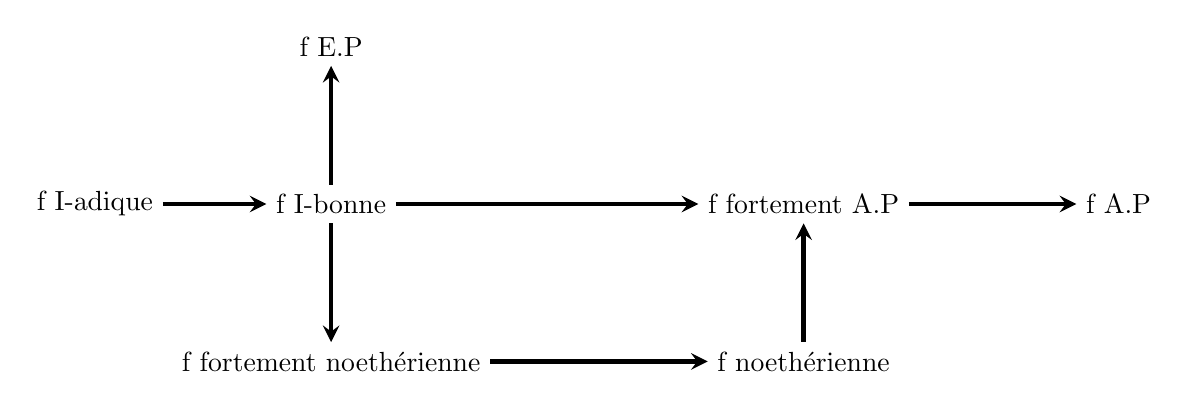
\begin{tikzpicture}
					\node (A) at (-1,0) {f I-adique};
					\node (B) at (2,0) {f I-bonne};
					\node (C) at (2,-2) {f fortement noethérienne};
					\node (D) at (8,-2) {f noethérienne};
					\node (E) at (12,0) {f A.P};
					\node (F) at (8,0) {f fortement A.P};
					\node (G) at (2,2) {f E.P};
					% Dessin des flèches avec des modifications pour les rendre plus visibles
					\draw[->, ultra thick, >=stealth] (A) -- (B);
					\draw[->, ultra thick, >=stealth] (B) -- (C);
					\draw[->, ultra thick, >=stealth] (B) -- (F);
					\draw[->, ultra thick, >=stealth] (C) -- (D);
					\draw[->, ultra thick, >=stealth] (F) -- (E);
					\draw[<-, ultra thick, >=stealth] (F) -- (D);
					\draw[->, ultra thick, >=stealth] (B) -- (G);
		\end{tikzpicture}
	\end{center}
\end{maremarque}



